\documentclass[11pt]{report}
\usepackage[margin=1in]{geometry}
\usepackage{array}
\usepackage{longtable}
\usepackage{titlesec}
\usepackage{graphicx}
\usepackage{parskip}
\usepackage{glossaries}
\usepackage{datetime}
\usepackage{hyperref}
\usepackage{rotating}
\usepackage{float}
\usepackage[toc,page]{appendix}
\usepackage{wrapfig}

\titleformat{\chapter}{\Large\bfseries}{}{0pt}{\huge}
\titlespacing\chapter{0pt}{*1}{*1}
\titlespacing\section{0pt}{*0}{-\parskip}
\titlespacing\subsection{0pt}{*0}{-\parskip}
\titlespacing\paragraph{0pt}{*0}{*3}

\newcolumntype{a}[1]{>{\centering}p{#1}}

\newcommand*{\TitleFont}{
      \usefont{\encodingdefault}{\rmdefault}{b}{n}
      \fontsize{24}{36}
      \selectfont
}
\newcommand*{\SubtitleFont}{
      \usefont{\encodingdefault}{\rmdefault}{}{n}
      \fontsize{12}{12}
      \selectfont
}
\newcommand{\thickline}{\rule{\textwidth}{1.6pt}}
\newcommand{\thinline}{\rule{\textwidth}{0.4pt}}
\newcommand{\novspace}{\vspace*{-\baselineskip}\vspace*{4pt}}
\renewcommand{\dateseparator}{-}
\let\oldtitle\title
\newcommand{\fulltitle}[2]{\oldtitle{\thickline \\ \novspace \thinline \\ \TitleFont {#1} \thinline \\ \novspace \thickline #2}}
\renewcommand{\title}[1]{\fulltitle{#1}{}}
\newcommand{\titleandsubtitle}[2]{\fulltitle{#1}{\\ \SubtitleFont{#2}}}
\newcommand{\tableoffiguresandtables}{\listoffigures\begingroup\let\clearpage\relax\listoftables\endgroup}
\newcommand{\textrotate}[1]{\begin{turn}{-90}#1\end{turn}}
\newcommand{\signature}[1]{\\Signature: & & Date: & \\ \cline{2-2} \cline{4-4}	& #1 & & YYYY-MM-DD \tabularnewline}
\newcommand{\signatures}{\begin{tabular}{ca{8cm}ca{4cm}c}\signature{Evan Milton}\signature{Josh DeWitt}\signature{Chad Staley}\signature{James Gehringer}\end{tabular}}
\newcommand{\minutesessentials}[8]{\section{Meeting #1}
\begin{tabular}{llc}
	Date & #2 & \\
	Time & #3 & \\
	Location & #4 & \\
	Attendance & Evan Milton & #5 \\
	& Josh DeWitt & #6 \\
	& Chad Staley & #7 \\
	& James Gehringer & #8 \\
\end{tabular}}
\newcommand{\minutesdetails}[2]{\paragraph{Agenda}\begin{enumerate}#1\end{enumerate}\paragraph{Decisions Reached}\begin{enumerate}#2\end{enumerate}}

\hypersetup{
	colorlinks,
	citecolor=black,
	filecolor=black,
	linkcolor=black,
	urlcolor=black
}

\author{
	Josh DeWitt \\
	Computer and Electronics Engineering \\
	University of Nebraska-Lincoln \\
	Computer Engineering, minor in Computer Science \\
	Mathematics
}
\date{\yyyymmdddate\today}

\newacronym{2d}{2-D}{Two-Dimensional}
\newacronym{3d}{3-D}{Three-Dimensional}
\newacronym{aon}{AON}{Activity On Node}
\newacronym{arm}{ARM}{Advanced RISC Machines}
\newacronym{bom}{BOM}{Bill of Materials}
\newacronym{cad}{CAD}{Computer-Aided Design}
\newacronym{ceen}{CEEN}{Computer and Electronics Engineering}
\newacronym{cnc}{CNC}{Computer Numerical Control}
\newacronym{cpu}{CPU}{Central Processing Unit}
\newacronym{dmm}{DMM}{Digital Multi-Meter}
\newacronym{drc}{DRC}{Design Rules Check}
\newacronym{dvi}{DVI}{Digital Visual Interface}
\newacronym{eco}{ECO}{Engineering Change Order}
\newacronym{ecr}{ECR}{Engineering Change Request}
\newacronym{gpio}{GPIO}{General Purpose Input/Output}
\newacronym{led}{LED}{Light Emitting Diode}
\newacronym{lrc}{LRC}{Linear Responsibility Chart}
\newacronym{pcb}{PCB}{Printed Circuit Board}
\newacronym{pi}{Pi}{Raspberry Pi}
\newacronym{pcsc}{PCSC}{Project Common Success Criteria}
\newacronym{pssc}{PSSC}{Project Specific Success Criteria}
\newacronym{tcpip}{TCP/IP}{Transmission Control Protocol/Internet Protocol}
\newacronym{ti}{TI}{Texas Instruments}
\newacronym{wbs}{WBS}{Work Breakdown Structure}
\newacronym{xp}{XP}{Extreme Programming}

\titleandsubtitle{CNC Interface \\ Firmware Listing and Software Design Review}{Design Homework Four}

\begin{document}
\maketitle

\chapter{Firmware Listing and Software Design Review}

\section{Introduction}
The \gls{cnc} Interface is a project to drive a \gls{cnc} using a simple user interface and no need for installing drivers.
Additionally, the \gls{cnc} Interface will not be plugged into the computer, but will be controlled through the network instead.
The focus of software design for this project was to allow development from day one, not requiring any of the project's hardware to begin.
To achieve this goal, a test-driven development approach was adopted, meaning unit tests that verify project success are created before any application code is written.
This approach has allowed the software development to stay on track and not be pushed off until the end of the project.

\section{C2000 Software Design Considerations}
In this project, the \gls{ti} C2000 Piccolo microcontroller was chosen over the cheaper MSP430 because of more device support and available libraries.
The libraries provide an abstraction to the hardware registers allowing faster coding for the device. 

\subsection{Memory Model}
\begin{wraptable}{r}{8cm}
	\vspace{-18pt}
	\caption{C2000 Memory Map}
	\label{tab:memory-map}
	\centering
	{\footnotesize
	\begin{tabular}{rl|c|c|} 
		\hline\hline
		&& Data Space & Program Space \\ \cline{3-4}
		0x00&0000 & \multicolumn{2}{c|}{M0 Vector RAM} \\ \cline{3-4}
		0x00&0040 & \multicolumn{2}{c|}{Boot Stack, RAM Functions} \\ \cline{3-4}
		0x00&0400 & \multicolumn{2}{c|}{Program Stack} \\ \cline{3-4}
		0x00&0600 & \multicolumn{2}{c|}{Global Variables} \\ \cline{3-4}
		0x00&0800 & Peripheral Frame 0 & Reserved \\ \cline{3-4}
		0x00&0D00 & Interrupt Table & Reserved \\ \cline{3-4}
		0x00&0E00 & Peripheral Frame 0 & Reserved \\ \cline{3-4}
		0x00&2000 & \multicolumn{2}{c|}{Reserved} \\ \cline{3-4}
		0x00&6000 & Peripheral Frame 1 & Reserved \\ \cline{3-4}
		0x00&7000 & Peripheral Frame 2 & Reserved \\ \cline{3-4}
		0x00&8000 & \multicolumn{2}{c|}{L0 SARAM} \\ \cline{3-4}
		0x00&9000 & \multicolumn{2}{c|}{Reserved} \\ \cline{3-4}
		0x3D&7800 & \multicolumn{2}{c|}{User OTP} \\ \cline{3-4}
		0x3D&7C00 & \multicolumn{2}{c|}{Reserved} \\ \cline{3-4}
		0x3F&0000 & \multicolumn{2}{c|}{Flash Program Code, Static Data} \\ \cline{3-4}
		0x3F&7FF6 & \multicolumn{2}{c|}{Flash Program Boot Location} \\ \cline{3-4}
		0x3F&7FF8 & \multicolumn{2}{c|}{128-bit Password} \\ \cline{3-4}
		0x3F&8000 & \multicolumn{2}{c|}{L0 SARAM} \\ \cline{3-4}
		0x3F&9000 & \multicolumn{2}{c|}{Reserved} \\ \cline{3-4}
		0x3F&E000 & \multicolumn{2}{c|}{Boot ROM} \\ \cline{3-4}
		\hline
	\end{tabular}
	}
\end{wraptable}
This slightly more expensive microcontroller has 12\gls{kb} of \gls{ram} and 64\gls{kb} of Flash allowing ample space for the project's code, along with 2\gls{kb} of \gls{otp} and 16\gls{kb} of factory-programmed \gls{rom} containing power-on boot-loading software and standard math-related tables, like sine and cosine waveforms.
Table ~\ref{tab:memory-map} shows the C2000's memory map according to the datasheet\cite{piccolo} and the linker command file for the release configuration.
Note that each memory address is 2 bytes. 
An alternate configuration exists that puts all code in \gls{ram}, but this configuration is only used for debugging because it is faster to load a new program into \gls{ram}.
Frequently executed code copied from flash into \gls{ram} at startup to allow power savings and ensure that it is fetched with 0 wait states on interrupt.

\subsection{C2000 Peripheral Usage}
The project makes use of the \gls{spi} for communication with the \gls{pi} during normal operation.
\gls{spi} was chosen because of the high-bandwidth achievable, already verified to work with a 1MHz clock using non-ideal wire jumpers.
The \gls{pi} communicates with the C2000 through \gls{uart} at startup for bootloader functions.
\gls{uart} was chosen because the boot \gls{rom} code defaults to interfacing with the \gls{uart} for serial bootloading.
\gls{gpio} pins are used to drive the direction lines for the motors, generate the stepper motor pulse trains, and read the status of the home and emergency stop signals.

\subsection{C2000 Code Architecture}
The C2000 code base uses a combination of polling the \gls{spi} communication device and timer-based interrupt-driven code for generating pulse trains to the motors.
A second interrupt is generated whenever the emergency stop line transitions from high-to-low or low-to-high, in which case all motor movement is stopped as quickly as possible.
The pulse train generation is real-time and must execute code as soon as the auto-reloaded timer expires, so polling for \gls{spi} data can be preempted by the timer interrupt.
An alternate design would be to use interrupt priority and allow the timer to interrupt the \gls{spi} interrupt, however a polling scheme is less risky and is easier to code.
Because communication can be interrupted, the \gls{pi} will require the C2000 to respond back with a \gls{crc} to ensure that the entire communication block was received.
Figure ~\ref{fig:c2000-main} depicts the polling loop for the C2000 and figure ~\ref{fig:c2000-pulse} depicts the interrupt routine for the pulse train generation.

\subsection{Raspberry Pi Code Architecture}
The code written for the \gls{pi} is written to read and write to named Linux pipes, or \gls{fifo} files managed by the \gls{os}.
These services are written to constantly run, so running a g-code file requires writing to a pipe, not starting up a program.
The use of pipes allows to better modularize the code base and avoid duplication by factoring out common code into projects.

\subsection{Testing and Debugging}
All code for the project is written after unit tests have been created that can be run on any machine using the program make to verify all application logic before implementing on the \gls{pi} or C2000.
The exception is writing to hardware configuration registers which must be changed, programmed, and manually tested for correctness.
Once these low-level configurations are created and verified, they are kept in a stable state in git and will not undergo unnecessary changes.
Code is considered complete when it passes all unit tests, that is, no code is written unless a failing tests proves that it is required.
It follows that new functionality requires that tests are written first, and code is written to make the tests pass.

\section{Software Design Narrative}
The code written for this project is intended to be as modular as possible, avoiding duplication of functionality and increasing testability.
The project relies on free software including the Arch distribution of Linux\cite{archlinux} for the \gls{os} on the \gls{pi}, Apache for web hosting from the \gls{pi}, PHP for creating the back-end services that the website makes calls to, JQuery for creating dynamic web pages, and CuTest, a lightweight unit testing framework for C projects.
As shown in figure ~\ref{fig:sw-hierarchy}, the project contains four software modules: the website control, g-code interpreter, \gls{cnc} driver, and the motor scheduler.
Though not used during normal operation, a set of bash scripts grouped together to create a simple way to set up the \gls{pi} was created to be able to quickly set up the \gls{pi} and get ready for development.

\subsection{Website Control}
The website control project is written in HTML, CSS, JavaScript, and PHP and is the main interface between the user and the \gls{cnc}.
The website gives the user the ability to upload, delete, and run g-code files and configure the \gls{cnc}'s characteristics, like gearing ration, maximum speed, and maximum acceleration.
The website has been set up, outlined, and approximately 85\% written, with all written code being completely tested.

\subsection{g-code Interpreter}
The g-code interpreter project is written in C and is responsible for reading g-code line-by-line and interpreting it into instructions for the C2000 to generate the motor pulse trains.
The g-code interpreter listens to a pipe for g-code commands, which may come from a g-code file or directly from the website when the user is homing the machine, then writes to another pipe that is received by the \gls{cnc} driver.
At startup, the g-code interpreter is responsible for driving the state of the C2000, instructing it to home the \gls{cnc}.
The g-code interpreter relies heavily on mathematic formulas created by Josh DeWitt, so many unit tests have been written to ensure proper functionality.
The g-code interpreter has been outlined, flow-charted, and approximately 90\% written, with all written code being completely tested.

\subsection{CNC Driver}
The \gls{cnc} driver project is written in C and is responsible for managing communication channels between the \gls{pi} and C2000 through the \gls{spi} and \gls{uart}.
The g-code interpreter does not write to the \gls{spi} or \gls{uart} directly because these actions require root privileges, so this one project was created to allow a single, small program to run as root, while the larger, more frequently changing programs are run by regular users.
The \gls{cnc} driver listens to a pipe for commands to send to the C2000 and forwards them through \gls{spi}, verifying the \gls{crc} returned from the C2000.
The \gls{cnc} driver also looks for a special command that indicates that the next bytes will be \gls{ti} hex data and the program should reset the C2000 and bootload the device with new code.
The \gls{cnc} driver has been outlined, flow-charted, and 100\% written and tested.

\subsection{Motor Scheduler}
The motor scheduler project is written in C and is responsible for listening for commands from the \gls{pi} and generating the pulse trains to the motors.
The project is based off an algorithm that requires no floating point operations on the C2000 for generating pulses, saving resources and allowing better real-time performance.
The commands are accepted through \gls{spi} and are acknowledged with a \gls{crc}, with the command format specified in a C header file shared between the g-code interpreter and this project.
The motor scheduler has been outlined, flow-charted, and approximately 65\% written, with all written code being completely tested.

\section{Summary}
The \gls{cnc} Interface's software is currently on-time because of the development approaches involving test-driven development and well thought-out modular software architecture that makes changes simple and low-risk.
The software hierarchy is a modular design that takes advantage of the available features of the Linux \gls{os} for faster development.
To aid in rapid development and implementation all firmware upgrades to any component of the \gls{cnc} Interface can be made remotely.
A user can \gls{ssh} into the \gls{pi} and make changes to the website control, g-code interpreter, or \gls{cnc} driver projects directly and bootload new C2000 code over the \gls{uart}.
The software architecture created for this project is robust and encourages changes in improvements, while mitigating change risks through unit testing.


\begin{appendices}
	\chapter{Firmware Flowchart}

\begin{figure}[!ht]
	\centering
	\begin{minipage}{.45\textwidth}
		\centering
		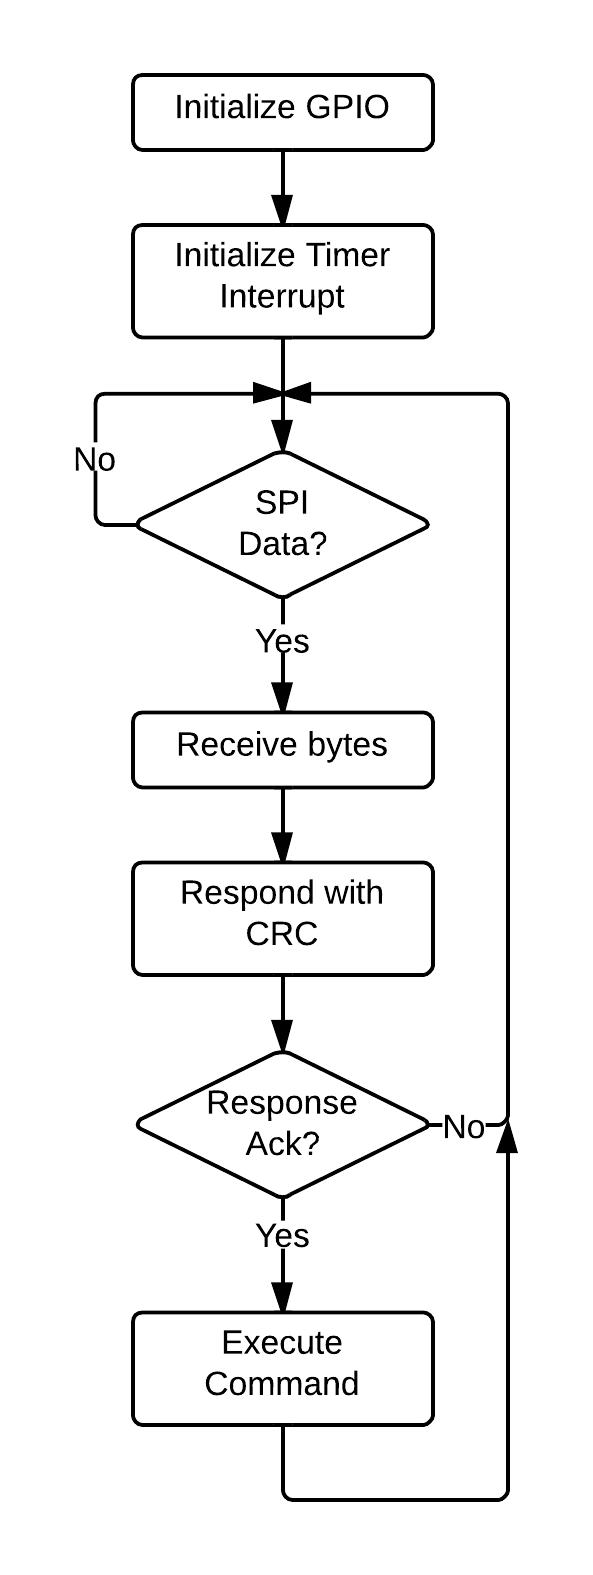
\includegraphics[width=.75\textwidth]{c2000-main.png}
		\caption{C2000 Main Program}
		\label{fig:c2000-main}
	\end{minipage}
	\begin{minipage}{.45\textwidth}
		\centering
		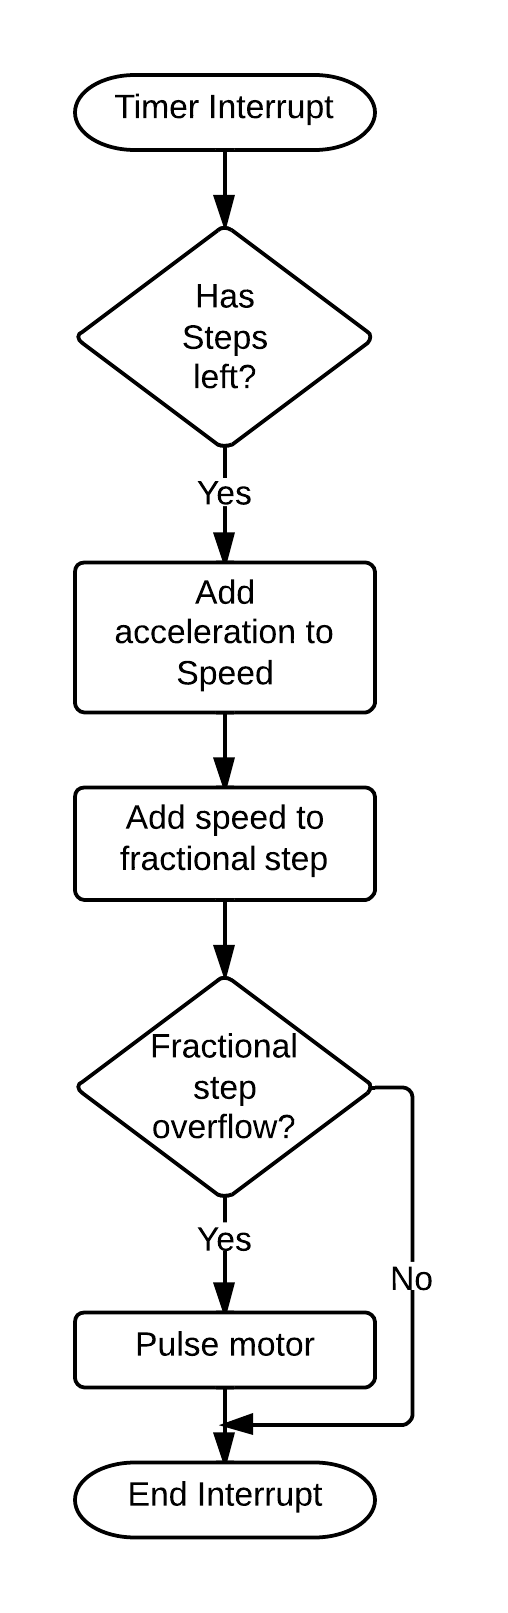
\includegraphics[width=.75\textwidth]{c2000-pulse.png}
		\caption{C2000 Pulse Generation}
		\label{fig:c2000-pulse}
	\end{minipage}
\end{figure}
	\chapter{Firmware Hierarchy}

\end{appendices}
\end{document}
